\subsection{Admin Interface}
\label{sec:admininterface}

The \ainterface[] is an extension of the \sinterface[], as the \ainterface[] is entered through the \sinterface[].
This makes sense because all persons given the permissions to enter the \ainterface[], will also be \astaff[] members.
There are two major fields\fixme{Foretr\ae kker noget andet her. M\aa{}ske bare classes?} of which the \admin[] has influence on, departments and persons.
These two are described in the following.

\subsubsection{Administrate Persons}
When an \admin[] enters the administrate persons window he/she is presented with a list of persons and a ``New Person'' button.
From this window the \admin[] can select an existing person and change the data of him or her 

\subsubsection{Administrate Departments}



\begin{figure}[htbp]
	\centering
		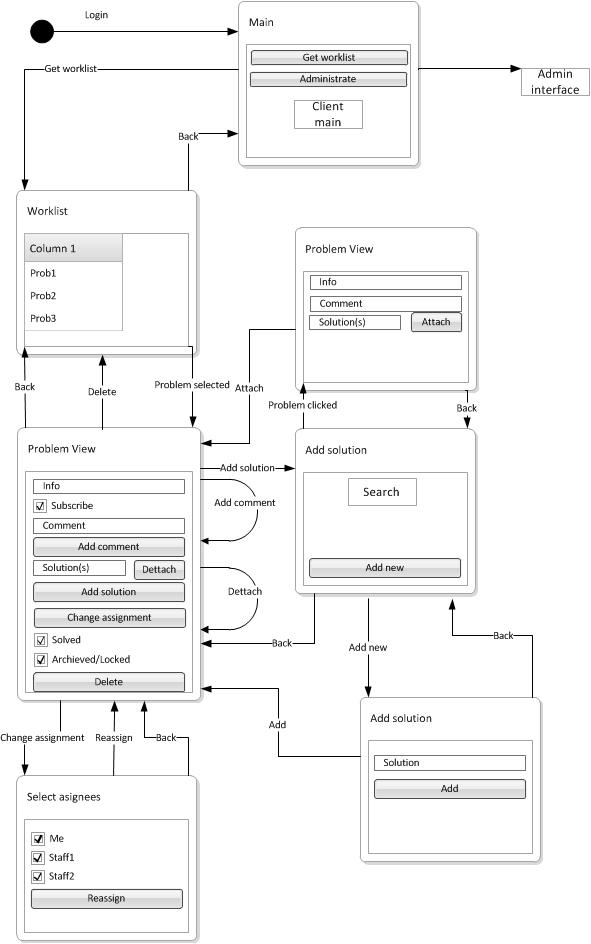
\includegraphics[width=0.75\textwidth]{input/application_domain_analysis/Navigation_DiagramStaff.jpg}
	\morscaption{\sinterface[c]}
	\label{fig:Navigation_DiagramStaff}
\end{figure}





\begin{comment}
\begin{itemize}
	\item department, including:
	\begin{itemize}
		\item categories
		\item tags
	\end{itemize}
	\item persons
\end{itemize}
\end{comment}